




%%%%%%%%%%%%%%%%%%%%%%%%%%%%%%%%%%%%%%%%%%%%%%%%%%%%%%%%%%%%%%%%%%%%%%%%%
%%%%%%%%%%%%%%%%%%%%%%%%%%%%%%%%%%%%%%%%%%%%%%%%%%%%%%%%%%%%%%%%%%%%%%%%%
%%%%%%%%%%%%%%%%%%%%%%%%%%%%%%%%%%%%%%%%%%%%%%%%%%%%%%%%%%%%%%%%%%%%%%%%%

\begin{frame}{What makes an estimator non-robust?  A tail sum.}

We show that \hspace{1em}
%
%\begin{align*}
$
%
\thetafunlin(\w^*) - \thetafun(\thetahat)  =
{\color{red}
    - \sum_{n=1}^{\lfloor \alpha N \rfloor} \infl_{(n)}
    =:  \noise \shape}
%
$
%\end{align*}
%
\hspace{1em} where \vspace{1em}

\begin{itemize}
\item The ``noise'' $\noise^2 \rightarrow \mathrm{Var}(\sqrt{N}\phi)$
    \begin{itemize}
        \item $\noise^2 = $ is the robust ``sandwich'' variance estimator
        \citep{hampel1986robustbook}
    \end{itemize}
\item The ``shape'' $\shape \le \sqrt{\alpha (1 - \alpha)}$
    determined by $\infl_n$ distribution
    \begin{itemize}
        \item $\shape$ converges to a nonzero constant
    \end{itemize}
\end{itemize}

\begin{center}
\begin{minipage}{0.65\linewidth}
\begin{tikzpicture}
    \onslide<1->{
    \node[anchor=south west,inner sep=0] (image) at (0,0) {
        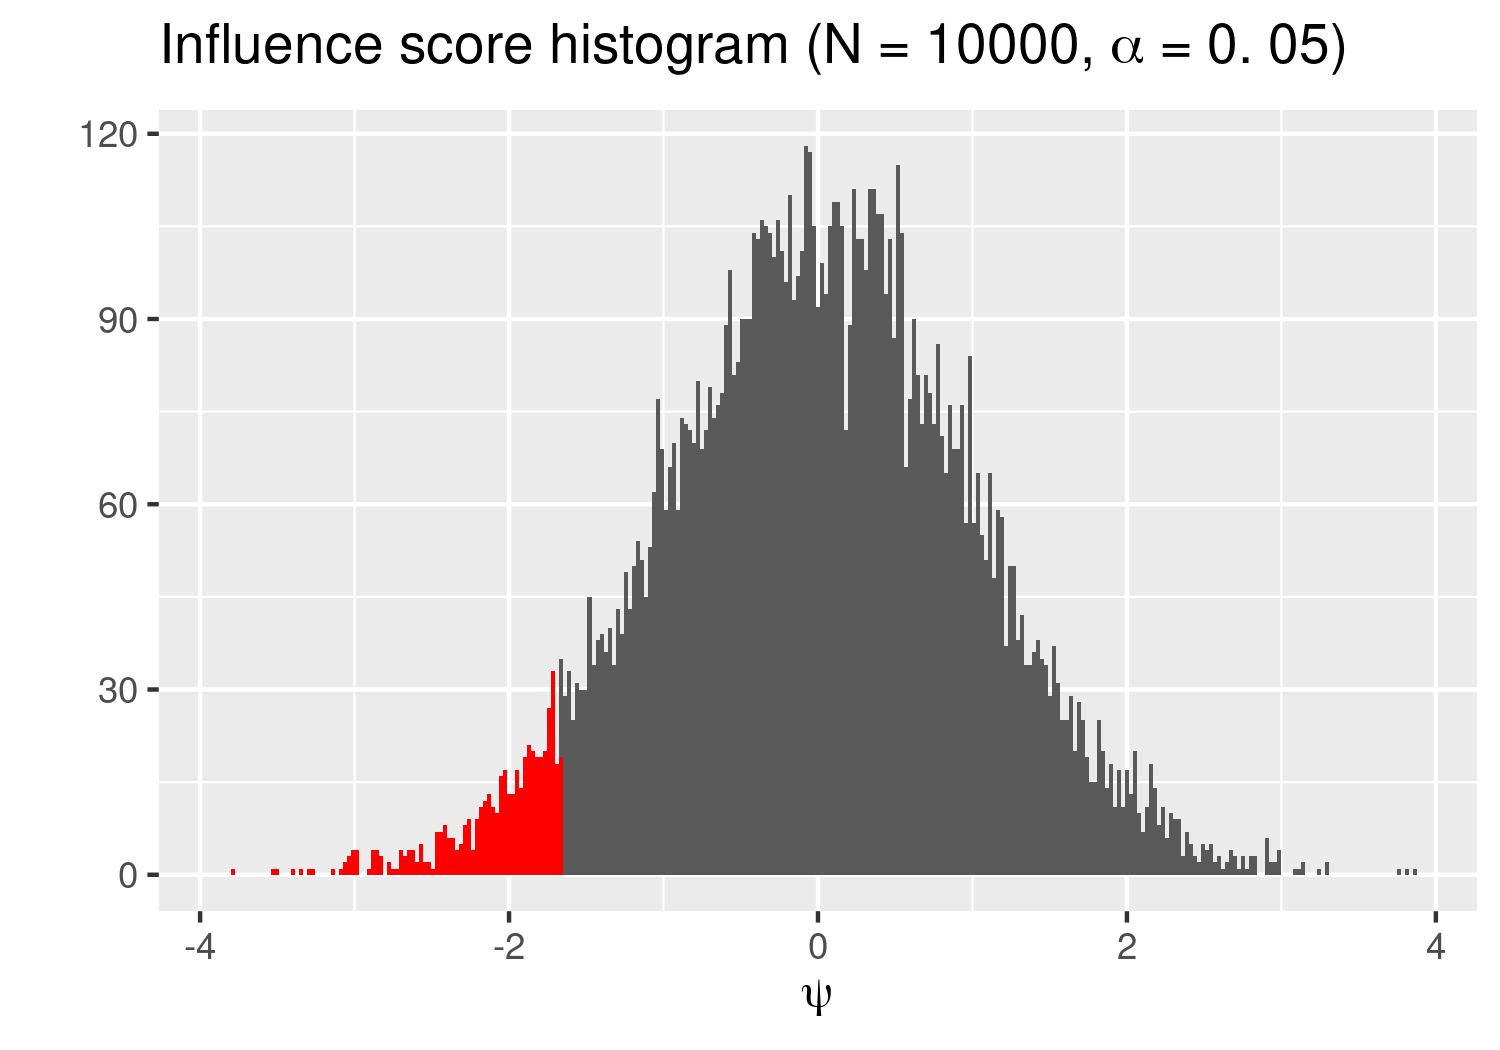
\includegraphics[width=0.98\textwidth]{static_figures/simple_infl_example.png}
    };
    }
    \onslide<1->{
    \begin{scope}[x={(image.south east)},y={(image.north west)}]
        \draw [stealth-stealth][thick][yellow](0.44, 0.4) -- (0.64, 0.4);
    \end{scope}
    \begin{scope}[x={(image.south east)},y={(image.north west)}]
        \draw (0.55,0.38) node[below,yellow][text width=3cm][align=center]
        % {\tiny $\noise$ is controlled by $\var{}{\sqrt{N}\phi(\thetahat)}$};
        {\small $\noise \approx $\\$\var{}{\sqrt{N}\phi(\thetahat)}$};
    \end{scope}
    }
    \onslide<1->{
    \begin{scope}[x={(image.south east)},y={(image.north west)}]
        \draw [stealth-][thick][red](0.3, 0.25) -- (0.3, 0.5);
    \end{scope}
    \begin{scope}[x={(image.south east)},y={(image.north west)}]
        \draw (0.25, 0.5) node[above][text width=3cm][align=center]
        {\small $-\sum_{n=1}^{\lfloor \alpha N \rfloor} \infl_{(n)}$};
    \end{scope}
    }
\end{tikzpicture}
\end{minipage}
\end{center}

\end{frame}



%%%%%%%%%%%%%%%%%%%%%%%%%%%%%%%%%%%%%%%%%%%%%%%%%%%%%%%%%%%%%%%%%%%%%%%%%
%%%%%%%%%%%%%%%%%%%%%%%%%%%%%%%%%%%%%%%%%%%%%%%%%%%%%%%%%%%%%%%%%%%%%%%%%
%%%%%%%%%%%%%%%%%%%%%%%%%%%%%%%%%%%%%%%%%%%%%%%%%%%%%%%%%%%%%%%%%%%%%%%%%

\begin{frame}[t]{Example.}

Report non-robustness if:
%
\begin{align*}
%
\thetafunlin(\w^*) - \thetafun(\thetahat)  = \noise \shape \ge \Delta
\quad\quad
\Leftrightarrow
\quad\quad
\frac{\Delta}{\noise} \le \shape.
%
\end{align*}
%
The \textbf{signal to noise ratio} $\frac{\Delta}{\noise}$
determines sensitivity to data dropping.

\hrulefill

\onslide<1->{
\footnotesize
\OHIEResultsTable{}
}
\vspace{-1em}
Let's analyze with $\alpha = 0.01 = 1\%$.
%
\begin{align*}
%
\begin{array}{rllrll}
\thetafun(\thetahat) ={}& -0.029  &\textrm{(Increase QOI by defn)}
    &   \Delta ={}& 0.029 \\
\noise ={}& 0.766 & \textrm{(Noise)}
        & \frac{1}{\sqrt{N}} \noise ={}& 0.005 &
        \textrm{(SE)} \\
\shape ={}& 0.046   &   \textrm{(Shape)}
    & \frac{1.96}{\sqrt{N}}  ={}& 0.0128
    & \rightarrow 0 \textrm{ as }N \rightarrow \infty\\
\shape \noise ={}& 0.035 & \textrm{(Data dropping sensitivity)}
    & \frac{1.96}{\sqrt{N}} \noise  ={}& 0.010
    & \textrm{(SE sensitivity)}\\
\end{array}
% %
\end{align*}
%
The noise is much larger than the signal $\Rightarrow$
Sensitive to data dropping.

\end{frame}


%%%%%%%%%%%%%%%%%%%%%%%%%%%%%%%%%%%%%%%%%%%%%%%%%%%%%%%%%%%%%%%%%%%%%%%%%
%%%%%%%%%%%%%%%%%%%%%%%%%%%%%%%%%%%%%%%%%%%%%%%%%%%%%%%%%%%%%%%%%%%%%%%%%
%%%%%%%%%%%%%%%%%%%%%%%%%%%%%%%%%%%%%%%%%%%%%%%%%%%%%%%%%%%%%%%%%%%%%%%%%

\begin{frame}[t]{Corollaries.}
%
Report non-robustness if:
%
\begin{align*}
%
\thetafunlin(\w^*) - \thetafun(\thetahat)  = \noise \shape \ge \Delta
\quad\quad
\Leftrightarrow
\quad\quad
\frac{\Delta}{\noise} \le \shape.
%
\end{align*}
%
The \textbf{signal to noise ratio} $\frac{\Delta}{\noise}$
determines sensitivity to data dropping.


\hrulefill

%\vspace{-1em}

\pause
\vspace{0.5em}
\textbf{Corollary:  Leave-$\lfloor \alpha N \rfloor$-out is different from standard errors.}\\
% \vspace{-0.4em}
% $1.96 / \sqrt{N} \ne \shape$
% \vspace{0.5em}
Standard errors reject when
$\frac{\Delta}{\noise} \le \frac{1.96}{\sqrt{N}} \ne \shape$.

\pause
\vspace{0.5em}
\textbf{Corollary:  Statistical insignificance is asymptotically non-robust.}
%\vspace{-0.4em}

$\frac{1.96 \hat \sigma_\phi}{\sqrt{N}} \rightarrow 0 \le \shape$.

\pause
\vspace{0.5em}
\textbf{Corollary:  Leave-$\lfloor \alpha N \rfloor$-out robustness does not vanish as $N \rightarrow \infty$.}\\
% \vspace{-0.4em}
%
Both $\shape$ and $\noise$ typically converge to nonzero constants.

\pause
\vspace{0.5em}
\textbf{Corollary:  Non-robustness possible even with correct specification.}
%\vspace{-0.4em}
% {\small The noise $\noise$ may be larger than the effect
% $\Delta$ you're trying to measure.}
%
% \pause
% \vspace{0.5em}
% \textbf{Corollary:  Gross outliers primarily affect robustness
% through $\noise$.}
% %\vspace{-0.4em}
% See paper for more details.

\pause
\vspace{0.5em}
\textbf{Corollary:  To robustify, reduce the noise or increase
the signal.}

\end{frame}
